\documentclass[12pt]{article}
\usepackage[margin=1in]{geometry}
\usepackage{enumitem}
\usepackage{amsmath}
\usepackage{graphicx}
\usepackage{hyperref}
\usepackage{listings}
\usepackage{xcolor}

% Header and Footer Configuration
\usepackage{fancyhdr}
\usepackage{lastpage}

\setlength{\headheight}{14pt}

\def\myheadertitle{CS 4513 - Database Management: Homework 3 - Problem 1}

\pagestyle{fancy}
\fancyhead{} % clear all header fields
\fancyhead[CO,CE]{\textsc{\myheadertitle}}
\fancyfoot{} % clear all footer fields
\fancyfoot[LO,RE]{\today}
\fancyfoot[RO,LE]{\thepage/\pageref*{LastPage}}
\renewcommand{\headrulewidth}{0.0pt}
\renewcommand{\footrulewidth}{0.0pt}

% First page style (for title page)
\fancypagestyle{firststyle}
{
   \fancyhf{}
   \fancyfoot[L]{\today}
   \fancyfoot[R]{\thepage/\pageref*{LastPage}}
}

% Code listing settings
\lstset{
    basicstyle=\ttfamily\small,
    breaklines=true,
    frame=single,
    numbers=left,
    numberstyle=\tiny\color{gray},
    captionpos=b,
    tabsize=2,
    showstringspaces=false
}

\begin{document}

% Cover Page
\begin{titlepage}
\thispagestyle{empty}
\centering
\vspace*{2cm}

\begin{flushleft}
{\Large \textbf{GROUP NUMBER:} Group 22}\\[0.5cm]
{\Large \textbf{GROUP MEMBERS:} Colby Frison, Brayden Garner, Brendan Ford, Jackson Dunlap}\\[0.5cm]
{\Large \textbf{GRADED HOMEWORK NUMBER:} 3}\\[0.5cm]
{\Large \textbf{COURSE:} CS/DSA-4513 - DATABASE MANAGEMENT}\\[0.5cm]
{\Large \textbf{SECTION:} 002}\\[0.5cm]
{\Large \textbf{SEMESTER:} FALL 2025}\\[0.5cm]
{\Large \textbf{INSTRUCTOR:} EGAWATI PANJEI}\\[0.5cm]
{\Large \textbf{SCORE:} }\\[2cm]
\end{flushleft}

\vfill

\end{titlepage}

% Table of Contents
\tableofcontents
\newpage

\section{Problem 1: JDBC and Stored Procedures (GQ1)}

\subsection{Problem Description}

Write a Java program using JDBC and Azure SQL Database to manage a relational database with the following schema:

\begin{itemize}
    \item \textbf{Passenger} (pid: integer, pname: string, tier: string, age: integer)
    \item \textbf{Pilot} (pIid: integer, pIname: string, hours: real)
    \item \textbf{Flight} (fnum: string, origin: string, destination: string, dep\_time: string, arrival\_time: string, pIid: integer)
    \item \textbf{Booking} (pid: integer, fnum: string)
\end{itemize}

\noindent The program provides a menu-driven interface to perform the following operations on the Pilot relation:

\begin{enumerate}
    \item \textbf{Insert a Pilot (Hours Based on Average Flight Time):} Insert a new pilot with hours calculated as the average flight time of all flights.
    
    \item \textbf{Insert a Pilot (Hours Based on Passenger Tier):} Insert a new pilot with hours calculated as the average flight time of flights piloted by pilots who have at least one passenger of a specified tier.
    
    \item \textbf{Display All Pilots:} Display all records in the Pilot table sorted by pIid.
    
    \item \textbf{Quit:} Exit the program.
\end{enumerate}

\subsection{Implementation Overview}

\subsubsection{Transact-SQL Stored Procedures}

Two stored procedures were created in Azure SQL Database to implement Options 1 and 2:

\paragraph{InsertPilotAvgFlightTime}
Accepts \texttt{pIid} and \texttt{pIname} as parameters. Calculates hours as the average flight time of all flights by using \texttt{DATEDIFF(MINUTE, dep\_time, arrival\_time)} divided by 60.0. Uses \texttt{ISNULL()} to return 0 if no flights exist.

\paragraph{InsertPilotByPassengerTier}
Accepts \texttt{pIid}, \texttt{pIname}, and \texttt{tier} as parameters. Calculates hours as the average flight time of flights piloted by pilots who have at least one passenger of the specified tier. Uses same time calculation and NULL handling as the first procedure.

\subsubsection{Java JDBC Implementation}

The Java program uses JDBC to connect to Azure SQL Database and provides a menu-driven interface. Key features:
\begin{itemize}
    \item Uses \texttt{CallableStatement} to execute stored procedures
    \item Uses \texttt{Statement} and \texttt{ResultSet} to query and display pilot data
    \item Continues until user selects Option 4 (Quit)
    \item Includes proper exception handling for SQL errors
\end{itemize}

\newpage
\section{Compilation and Execution}

\subsection{Compilation}

The Java program was compiled using:

{\footnotesize
\begin{verbatim}
javac -cp ".;sqljdbc_13.2.1.0_enu\sqljdbc_13.2\enu\jars\mssql-jdbc-13.2.1.jre11.jar" 
      Problem1.java
\end{verbatim}
}

\subsection{Stored Procedure Creation}

The Transact-SQL stored procedures were created in Azure SQL Database by executing the \texttt{Problem1\_StoredProcedures.sql} file in the Azure SQL Query Editor.

\subsection{Program Execution}

The program was executed using:

{\footnotesize
\begin{verbatim}
java -cp ".;sqljdbc_13.2.1.0_enu\sqljdbc_13.2\enu\jars\mssql-jdbc-13.2.1.jre11.jar" 
     Problem1
\end{verbatim}
}

\newpage
\section{Test Execution Results}

\subsection{Program Start and Main Menu}

\begin{figure}[h]
\centering
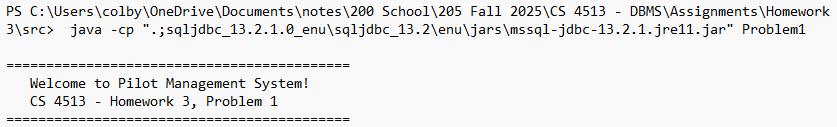
\includegraphics[width=0.85\textwidth]{../../../Screenshots/Problem1/Other/Program_start.png}
\caption{Program Start - Connection to Azure SQL Database}
\label{fig:program_start}
\end{figure}

\begin{figure}[h]
\centering
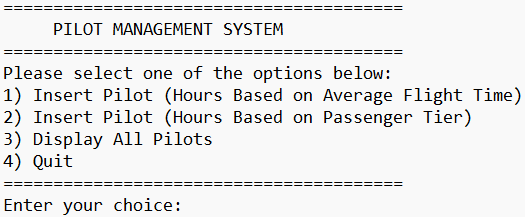
\includegraphics[width=0.85\textwidth]{../../../Screenshots/Problem1/Other/Mainmenu.png}
\caption{Main Menu - Four menu options displayed}
\label{fig:main_menu}
\end{figure}

The program successfully connects to Azure SQL Database and displays the menu-driven interface with all four options.

\newpage
\subsection{Option 1: Insert Pilot Based on Average Flight Time}

Option 1 inserts a new pilot with hours calculated based on the average flight time of all flights in the database. The stored procedure \texttt{InsertPilotAvgFlightTime} is called with pilot ID and name as parameters.

\subsubsection{Execution 1}

\begin{figure}[h]
\centering
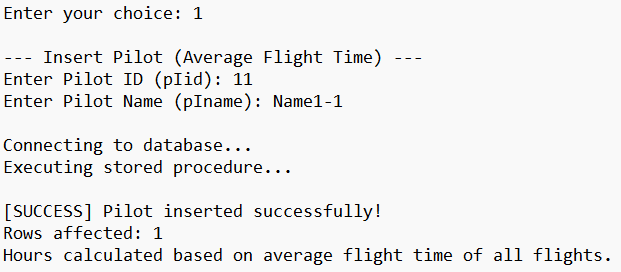
\includegraphics[width=0.8\textwidth]{../../../Screenshots/Problem1/Option1/Option1-1.png}
\caption{Option 1 Execution 1 - Inserting pilot with pIid=100, pIname=name1}
\label{fig:option1_exec1}
\end{figure}

\begin{figure}[h]
\centering
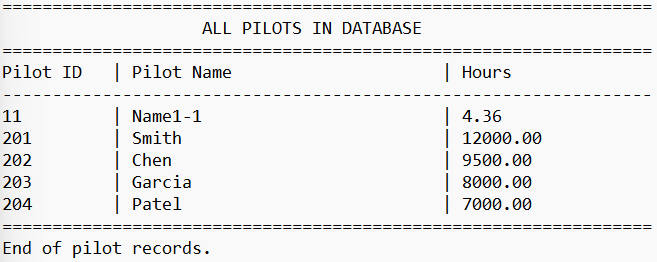
\includegraphics[width=0.8\textwidth]{../../../Screenshots/Problem1/Option1/Option1-1_result.png}
\caption{Option 1 Result 1 - Pilot table after insertion (Option 3 display)}
\label{fig:option1_result1}
\end{figure}

\textbf{Note:} Pilots 201-204 (Smith, Chen, Garcia, Patel) are from the original dataset. The new pilot (Name1-X) shows the calculated hours based on average flight time.

\newpage
\subsubsection{Execution 2}

\begin{figure}[h]
\centering
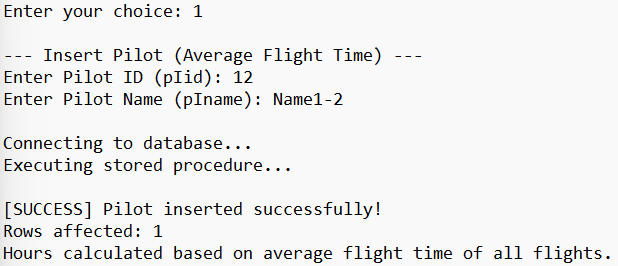
\includegraphics[width=0.8\textwidth]{../../../Screenshots/Problem1/Option1/Option1-2.png}
\caption{Option 1 Execution 2 - Inserting another pilot with average flight time calculation}
\label{fig:option1_exec2}
\end{figure}

\begin{figure}[h]
\centering
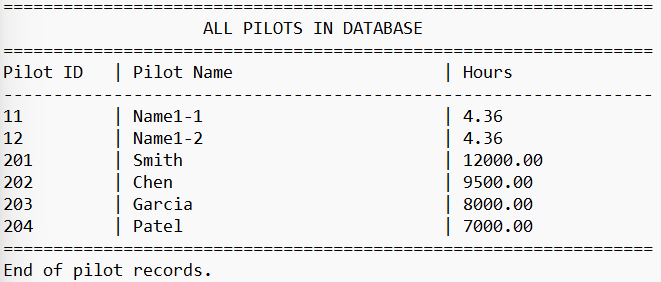
\includegraphics[width=0.8\textwidth]{../../../Screenshots/Problem1/Option1/Option1-2_result.png}
\caption{Option 1 Result 2 - Pilot table showing both new insertions}
\label{fig:option1_result2}
\end{figure}

\newpage
\subsubsection{Execution 3}

\begin{figure}[h]
\centering
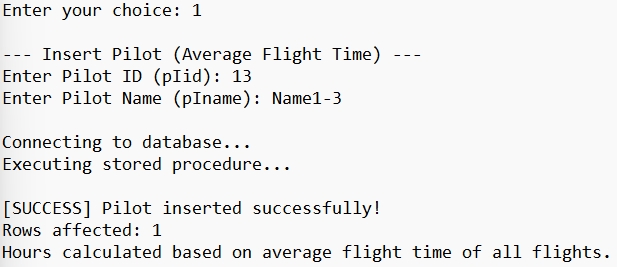
\includegraphics[width=0.8\textwidth]{../../../Screenshots/Problem1/Option1/Option1-3.png}
\caption{Option 1 Execution 3 - Third insertion using average flight time}
\label{fig:option1_exec3}
\end{figure}

\begin{figure}[h]
\centering
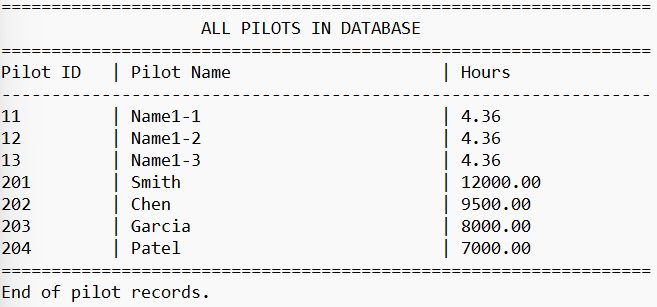
\includegraphics[width=0.8\textwidth]{../../../Screenshots/Problem1/Option1/Option1-3_result.png}
\caption{Option 1 Result 3 - Pilot table with all three new pilots from Option 1}
\label{fig:option1_result3}
\end{figure}

\textbf{Observation:} All three pilots inserted via Option 1 have the same hours value, demonstrating that the calculation is based on the current average flight time across all flights in the database.

\newpage
\subsection{Option 2: Insert Pilot Based on Passenger Tier}

Option 2 inserts a new pilot with hours calculated based on the average flight time of flights piloted by pilots who have at least one passenger of the specified tier. The stored procedure \texttt{InsertPilotByPassengerTier} is called with pilot ID, name, and tier as parameters.

\subsubsection{Execution 1 - Gold Tier}

\begin{figure}[h]
\centering
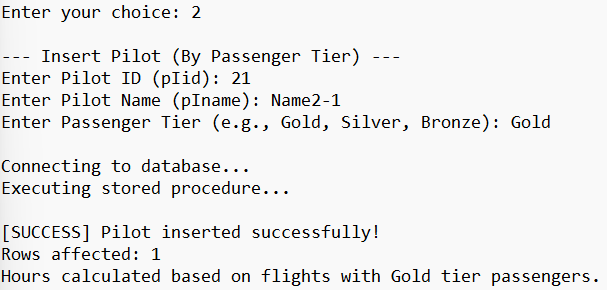
\includegraphics[width=0.8\textwidth]{../../../Screenshots/Problem1/Option2/Option2-1.png}
\caption{Option 2 Execution 1 - Inserting pilot based on Gold tier passengers}
\label{fig:option2_exec1}
\end{figure}

\begin{figure}[h]
\centering
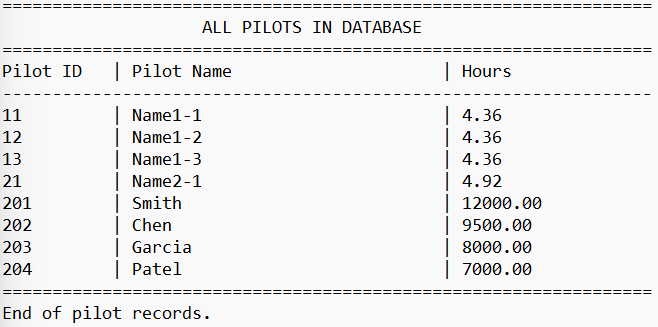
\includegraphics[width=0.8\textwidth]{../../../Screenshots/Problem1/Option2/Option2-1_result.png}
\caption{Option 2 Result 1 - Pilot table after Gold tier insertion}
\label{fig:option2_result1}
\end{figure}

\textbf{Note:} Pilots 201-204 (Smith, Chen, Garcia, Patel) and pilots 11-13 (Name1-X) are from the original dataset. The new pilot (Name2-X) show the insertion of pilot based on tier.


\newpage
\subsubsection{Execution 2 - Silver Tier}

\begin{figure}[h]
\centering
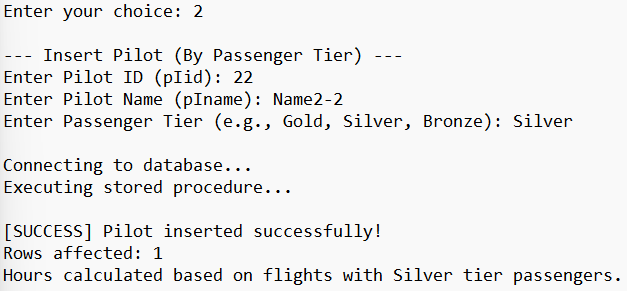
\includegraphics[width=0.8\textwidth]{../../../Screenshots/Problem1/Option2/Option2-2.png}
\caption{Option 2 Execution 2 - Inserting pilot based on Silver tier passengers}
\label{fig:option2_exec2}
\end{figure}

\begin{figure}[h]
\centering
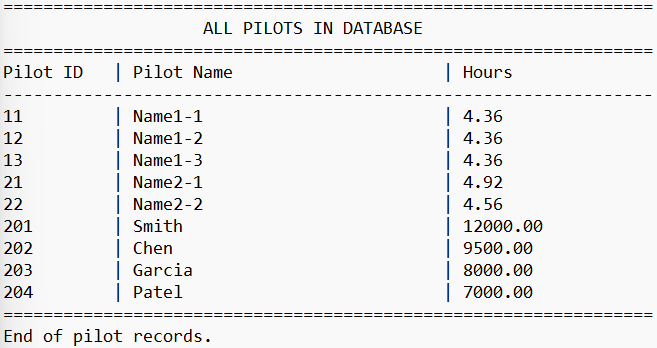
\includegraphics[width=0.8\textwidth]{../../../Screenshots/Problem1/Option2/Option2-2_result.png}
\caption{Option 2 Result 2 - Pilot table showing Silver tier calculation}
\label{fig:option2_result2}
\end{figure}

\newpage
\subsubsection{Execution 3 - Bronze Tier}

\begin{figure}[h]
\centering
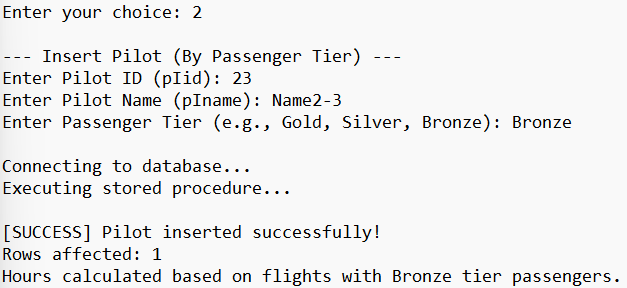
\includegraphics[width=0.8\textwidth]{../../../Screenshots/Problem1/Option2/Option2-3.png}
\caption{Option 2 Execution 3 - Inserting pilot based on Bronze tier passengers}
\label{fig:option2_exec3}
\end{figure}

\begin{figure}[h]
\centering
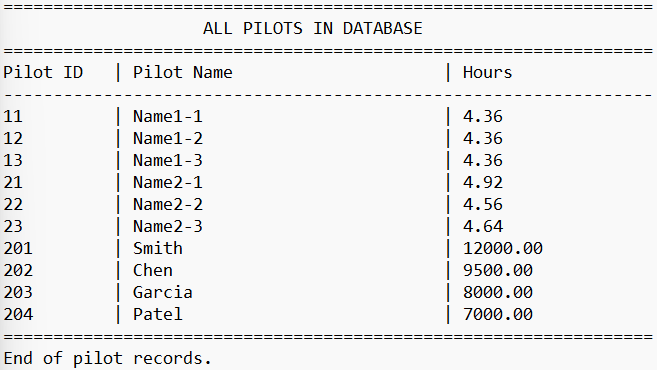
\includegraphics[width=0.8\textwidth]{../../../Screenshots/Problem1/Option2/Option2-3_result.png}
\caption{Option 2 Result 3 - Pilot table with all tier-based calculations}
\label{fig:option2_result3}
\end{figure}

\textbf{Observation:} Different passenger tiers produce different hours values, demonstrating that the tier-based calculation correctly filters flights based on passenger membership level.

\newpage
\subsection{Option 3: Display All Pilots}

Option 3 displays all pilots currently in the database sorted by pIid. This option was executed multiple times throughout testing to verify the results of Options 1 and 2 insertions.

\begin{figure}[h]
\centering
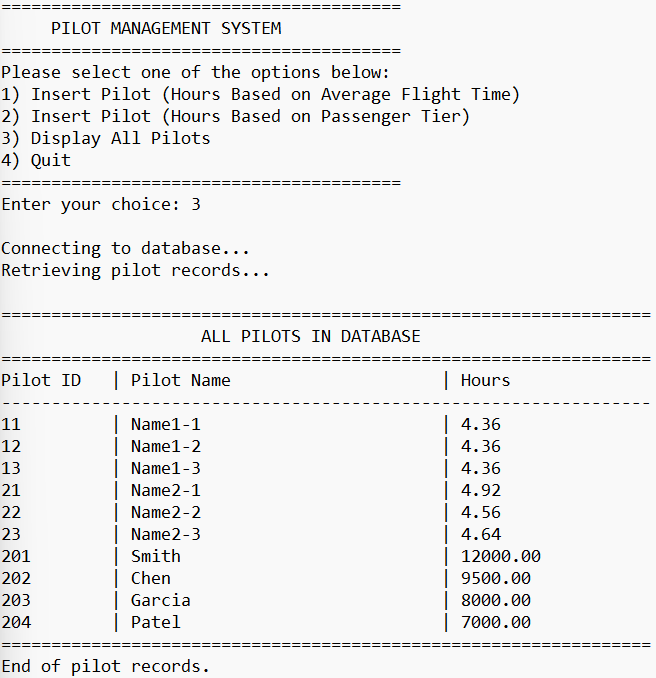
\includegraphics[width=0.85\textwidth]{../../../Screenshots/Problem1/Other/Option3_final.png}
\caption{Option 3 - Final display showing all pilots in database sorted by pIid}
\label{fig:option3_final}
\end{figure}

The final display shows:
\begin{itemize}
    \item Original pilots (IDs 201-204): Smith, Chen, Garcia, and Patel from the initial dataset
    \item New pilots from Option 1 (IDs 11-13): Name1-1, Name1-2, Name1-3 with hours based on average flight time
    \item New pilots from Option 2 (IDs 21-23): Name2-1 (Gold), Name2-2 (Silver), Name2-3 (Bronze) with hours based on tier
\end{itemize}

\newpage
\subsection{Option 4: Program Termination}

Option 4 allows the user to exit the program cleanly. When selected, the program displays a termination message and exits.

\begin{figure}[h]
\centering
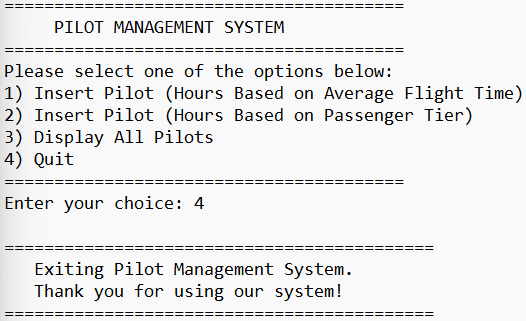
\includegraphics[width=0.85\textwidth]{../../../Screenshots/Problem1/Other/Option4.png}
\caption{Option 4 - Program termination with exit message}
\label{fig:option4}
\end{figure}

The program successfully terminates with an appropriate farewell message, demonstrating that the menu loop only exits when Option 4 is explicitly selected by the user.

\newpage
\section{Summary}

\subsection{Requirements Verification}

All requirements are met:

\begin{itemize}
    \item \textbf{JDBC Connection:} Program successfully connects to Azure SQL Database
    \item \textbf{Menu-driven interface:} Four-option menu displayed and functional
    \item \textbf{Program termination:} Program only exits when Option 4 is selected
    \item \textbf{Stored procedures:} Options 1 and 2 implemented as T-SQL stored procedures accepting required parameters (pIid, pIname, and tier for Option 2)
    \item \textbf{Flight time calculation:} Stored procedures calculate flight time by subtracting dep\_time from arrival\_time and converting to hours
    \item \textbf{Testing requirement:} Option 3 executed before and after each insertion to display changes
    \item \textbf{Execution count:} Options 1 and 2 each executed three times with different values
    \item \textbf{Option 4 execution:} Executed to verify proper program termination
    \item \textbf{Code comments:} Both Java and SQL files include detailed comments
\end{itemize}

\section{Conclusion}

The Java program and Transact-SQL stored procedures were successfully implemented and tested according to all assignment requirements. The implementation demonstrates:

\begin{itemize}
    \item Effective use of JDBC for database connectivity
    \item Proper implementation of stored procedures in T-SQL
    \item Menu-driven user interface with appropriate input/output handling
    \item Correct calculation of flight times and hours
    \item Comprehensive testing of all program features
\end{itemize}

\end{document}
